% JuliaCon proceedings template
\documentclass{juliacon}
\setcounter{page}{1}
\usepackage{caption}
\usepackage{csquotes}
\usepackage{amsmath}
%\bibliographystyle{juliacon}

\begin{document}

% **************GENERATED FILE, DO NOT EDIT**************

\title{ProbabilityBoundsAnalysis.jl:\\ an arithmetic of probabilities and sets of probabilities}

\author[1]{Ander Gray}
\author[1]{Scott Ferson}
\author[1, 2]{Edoardo Patelli}
\affil[1]{Institute for Risk and Uncertainty, University of Liverpool}
\affil[2]{Centre for Intelligent Infrastructure, University of Strathclyde}

\keywords{Julia, Probability, Uncertainty, Interval Arithmetic, Probabilistic Arithmetic}

\hypersetup{
pdftitle = {ProbabilityBoundsAnalysis.jl:\\ an arithmetic of probabilities and sets of probabilities},
pdfsubject = {JuliaCon 2019 Proceedings},
pdfauthor = {Ander Gray, Scott Ferson, Edoardo Patelli},
pdfkeywords = {Julia, Probability, Uncertainty, Interval Arithmetic, Probabilistic Arithmetic},
}



\maketitle

\begin{abstract}

Probability Bounds Analysis combines interval arithmetic with probability theory, and provides a representation of sets of distributions in structures called probability boxes (p-boxes), which generalise both distribution functions and intervals. P-boxes generally return interval bounds on all probabilistic quantities, for example samples, cdfs, and probability measures are all intervals. This framework also allows for the comprehensive propagation of probabilities through calculations in a rigorous way, in a similar fashion that interval arithmetic does for sets. As such, ProbabilityBoundsAnalysis.jl gives a rigorous arithmetic of random variables, where both marginal (univariate) and dependency information can be known, partially known or missing completely. We describe the main theoretical elements of probability bounds analysis, and describe a minimal implementation of the method and it's main algorithms in Julia.

\end{abstract}

\section{Introduction}
\label{sec:intro}


An arithmetic of probability distributions has held a long interest among mathematicians and scientists:
\begin{displayquote}
  A question asked by Kolmogorov, \\
  answered for the sum by Marakov, \\
  partially answered by Sklar and Frank (for which the copula was invented),\\
  made algorithmically available by Williamson, \\
  and generalised by others.
\end{displayquote}

\noindent Indeed it was Kolmogorov who originally asked about the result of a sum of two distributions without knowing their joint distribution. This was answered for the sum by Marakov \cite{makarov1982estimates}, who showed the result was a set of distributions and was able to provide bounds on this function. Sklar, Schweizer and Frank generalised this result to other (positive) binary operations \cite{frank1987best,schweizer2011probabilistic}. In this pursuit they created copulas, a general way to encode probabilistic dependence independently from marginals, and a now essential object used in probabilistic modelling. In his seminal dissertation \cite{williamson1989probabilistic}, Williamson described an algorithm for efficiently performing these arithmetic operations, which can give guaranteed bounds on probability distributions in terms of an upper and lower cdf. He called his method \textit{Probabilistic Arithmetic} and his sets of distributions \textit{Dependency Bounds}. Since then the method has been generalised \cite{ferson2015constructing,ferson1996whereof,ferson2004arithmetic} to most of the base binary and unary operations that would be present in a programming language. Probability Boxes (p-boxes) are the name now given to these structures, and Probability Bounds Analysis (PBA) the name of the method.

The goal of PBA can be stated as \textbf{to compute guaranteed bounds on functions of random variables given only partial knowledge of the input probability distributions and their dependencies}. That is to compute with partial knowledge about the input joint distribution. Ideally all of the available information about random variables should be used, but no more than what actually is available.

The idea of bounding probability has a very long tradition throughout the history of probability theory. George Boole \cite{boole1854investigation, hailperin1986boole} used the notion of interval bounds on probability. Chebyshev \cite{chebyshev1874valeurs} described bounds on a distribution when only the mean and variance of the variable are known, and Markov \cite{markoff1900question} found bounds on a positive variable when only the mean is known.  Fréchet \cite{frechet1935generalisation} discovered how to bound joint distributions solely from knowing the marginal distributions, without making independence assumptions. Bounding probabilities has continued to the present day, culminating into the modern theory of Imprecise Probabilities \cite{walley1991statistical, klir2013uncertainty, troffaes2014lower, augustin2014introduction}.

Imprecise probabilities is effectively a generalisation of probability theory where uncertainty can be expressed about the probability measure. This 
is particularly relevant when information is scarce, unreliable, vague, conflicting or imprecise. In such cases defining a unique probability distribution is difficult. P-boxes are one of many ways to describe a set of distributions, others include: Dempster-Shafer structures \cite{dempster2008upper,shafer1976mathematical}, random sets \cite{molchanov2005theory}, possibility distributions \cite{zadeh1978fuzzy,dubois1988possibility, hose2019possibilistic} and lower previsions \cite{troffaes2014lower}. These structures were discovered independently, but are often synonymous and can be translated from one to another, with different degrees of generality. Imprecise probabilities links all these theories into one. For a comprehensive overview of the theory, and a for a formal description of uncertainty and information in terms of these structures, \cite{klir2013uncertainty} is recommended. In that sense PBA is a part of imprecise probabilities but provides a framework for computing with p-boxes.



\iffalse
Probability bounds analysis is a combination of the methods of standard interval analysis \cite{moore1996interval, jaulin2001interval} and classical probability theory (see, inter alia, \cite{feller1968probability, feller1971probability}).  The idea of bounding probability has a very long tradition throughout the history of probability theory.  Indeed, George Boole \cite{boole1854investigation, hailperin1986boole} used the notion of interval bounds on probability.  Chebyshev \cite{chebyshev1874valeurs} described bounds on a distribution when only the mean and variance of the variable are known, and Markov \cite{markoff1900question} found bounds on a positive variable when only the mean is known.  Fréchet \cite{frechet1935generalisation} discovered how to make calculations with uncertain estimates of joint probabilities without making independence assumptions.  Bounding probabilities has continued to the present day \cite{walley1991statistical, klir2013uncertainty, troffaes2014lower, augustin2014introduction}, culminating into the modern theory of Imprecise Probabilities.

An arithmetic of probability distributions has held a long interest among mathematicians and engineers




Computations with probabilities are usually performed by Monte-Carlo style simulations, where essentially many random realisations of functions are required to be run. These sampling methods require many thousands of realisations to be accurate, and even then will only produce an approximation of the desired probabilistic quantity. In contrast, the methods ProbabilityBoundsAnalysis.jl are exact rather than approximate, and give no restriction to the distribution shape or dependency.
\fi


\section{Probability Boxes}
\label{sec:pboxes}

A probability box defines a set of distributions with the following three constrains: (1) interval bounds on the cumulative distribution function (cdf), (2) interval bound on the mean and variance, and (3) a collection of distribution families:

\begin{enumerate}
  \item $\begin{aligned}[t]
    \underline{F}(x) \leq F(x) \leq \overline{F}(x) \\%&&&& \text{(Bounds on the cdf)} \\
  \end{aligned}$
  \item $\begin{aligned}[t]
    \mu &\in [\underline{ \mu }, \overline{ \mu }]  \\%&&&& \text{(bounds on mean and variance)}\\
    \sigma^2 &\in [\underline{\sigma}^2 , \overline{\sigma}^2]
  \end{aligned}$
  \item $\begin{aligned}[t]
      F \in \bold{F} \\%&&&&&&& \text{(distribution family)} \\
  \end{aligned}$
  \end{enumerate}

\noindent That is, a random variable is a member of a p-box if its cdf $F$ falls within the cdf bounds of the p-box $F(x) \in [\underline{F}(x), \overline{F}(x)]$ for all x, its moments are inside the interval moments of the p-box, and it belongs to a family of distribution functions (e.g. normal, uniform) considered by the p-box. Some of the constraints may be missing. For example, if the distribution family is unknown then the set is defined solely from the cdf and moment bounds. Such p-boxes are sometimes called non-parametric, since its members do not have to belong to any particular class of distribution. Some constraints may also be inferred from others. For example, the interval moments may be bounded from the cdf bounds, and cdf may be bounded from moment information (explored further in section \ref{section:Moments}).

All of a p-box's probabilistic quantities are intervals. The cdf of a p-box may be found by: 

\begin{equation*}
  [\underline{F}(x), \overline{F}(x)] ,
\end{equation*}

\noindent a sample of the p-box may be drawn using the inverse cdfs: 

\begin{equation*}
  [\underline{F}^{-1}(\alpha), \overline{F}^{-1}(\alpha)]
\end{equation*}

\noindent where $\alpha \sim U(0,1)$ is a sample from a uniform distribution, and the probability measure\footnote{The probability measure is a function which returns the probability that the random variable is in some set} on some interval $U = [a, b]$ is bounded as follows:

\begin{align*}
  \underline{\mathbb{P}}(U) &= \text{max}(0, \underline{F}(b) - \overline{F}(a)) \\ 
  \overline{\mathbb{P}}(U)  &= \overline{F}(b) - \underline{F}(a) ,
\end{align*}

where the max operator is required when $\underline{F}(b) < \overline{F}(a)$. Note the same can be achieved by using the standard formula for finding the measure from the cdf, $\mathbb{P}(U) = F(b)- F(a)$, and using interval arithmetic.


\begin{figure*}[htp]

  \centering
  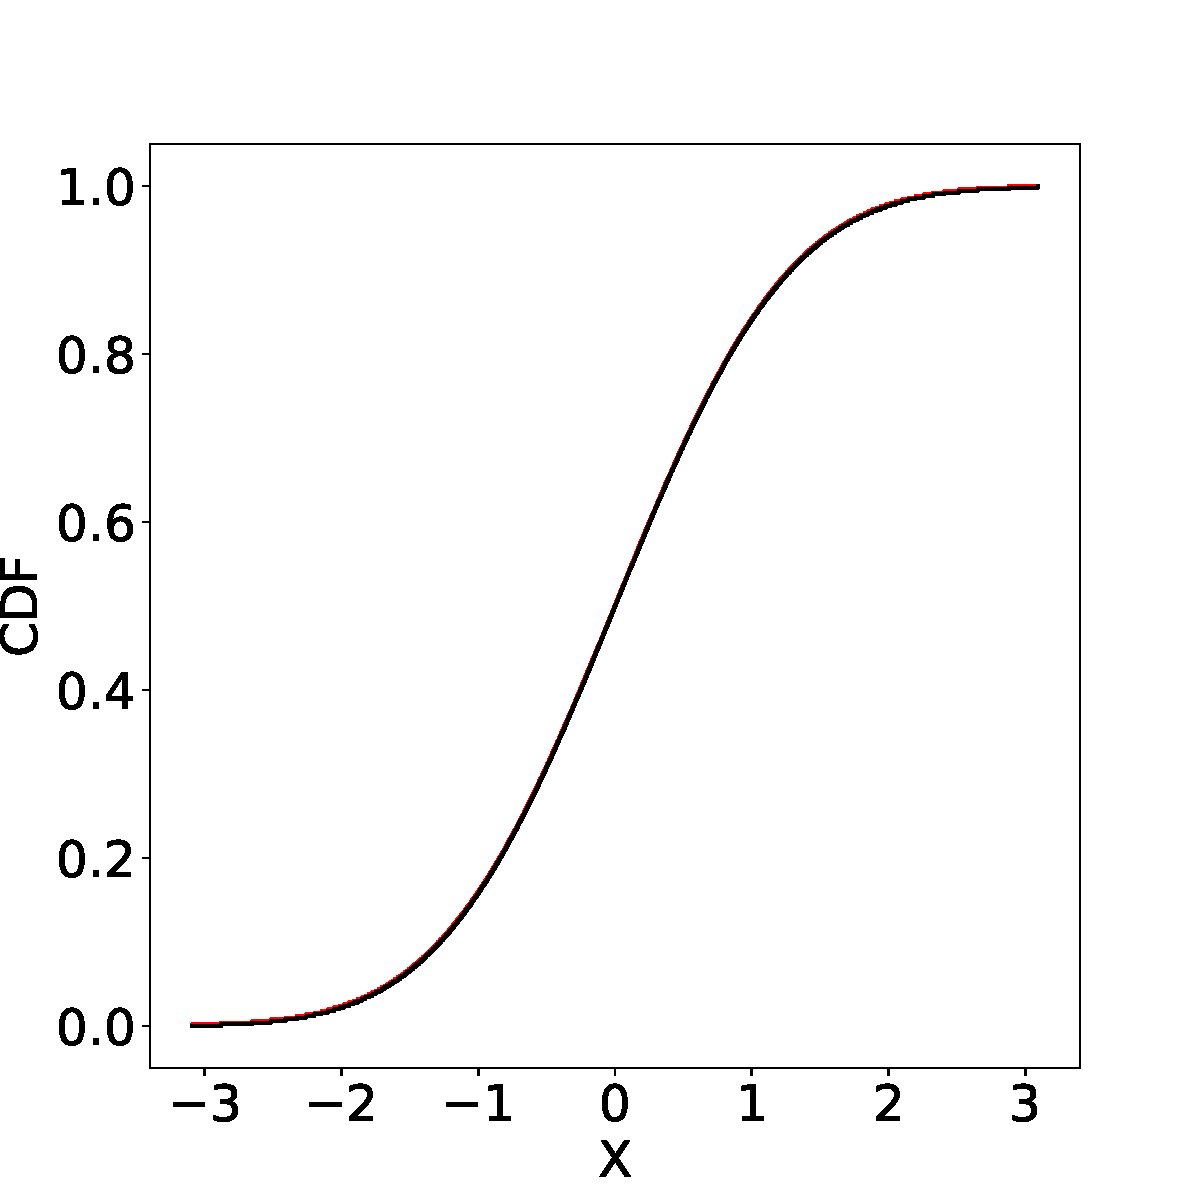
\includegraphics[width=.3\textwidth]{../examples/JuliaCon/fig1/fig1_dist.pdf}\hfill
  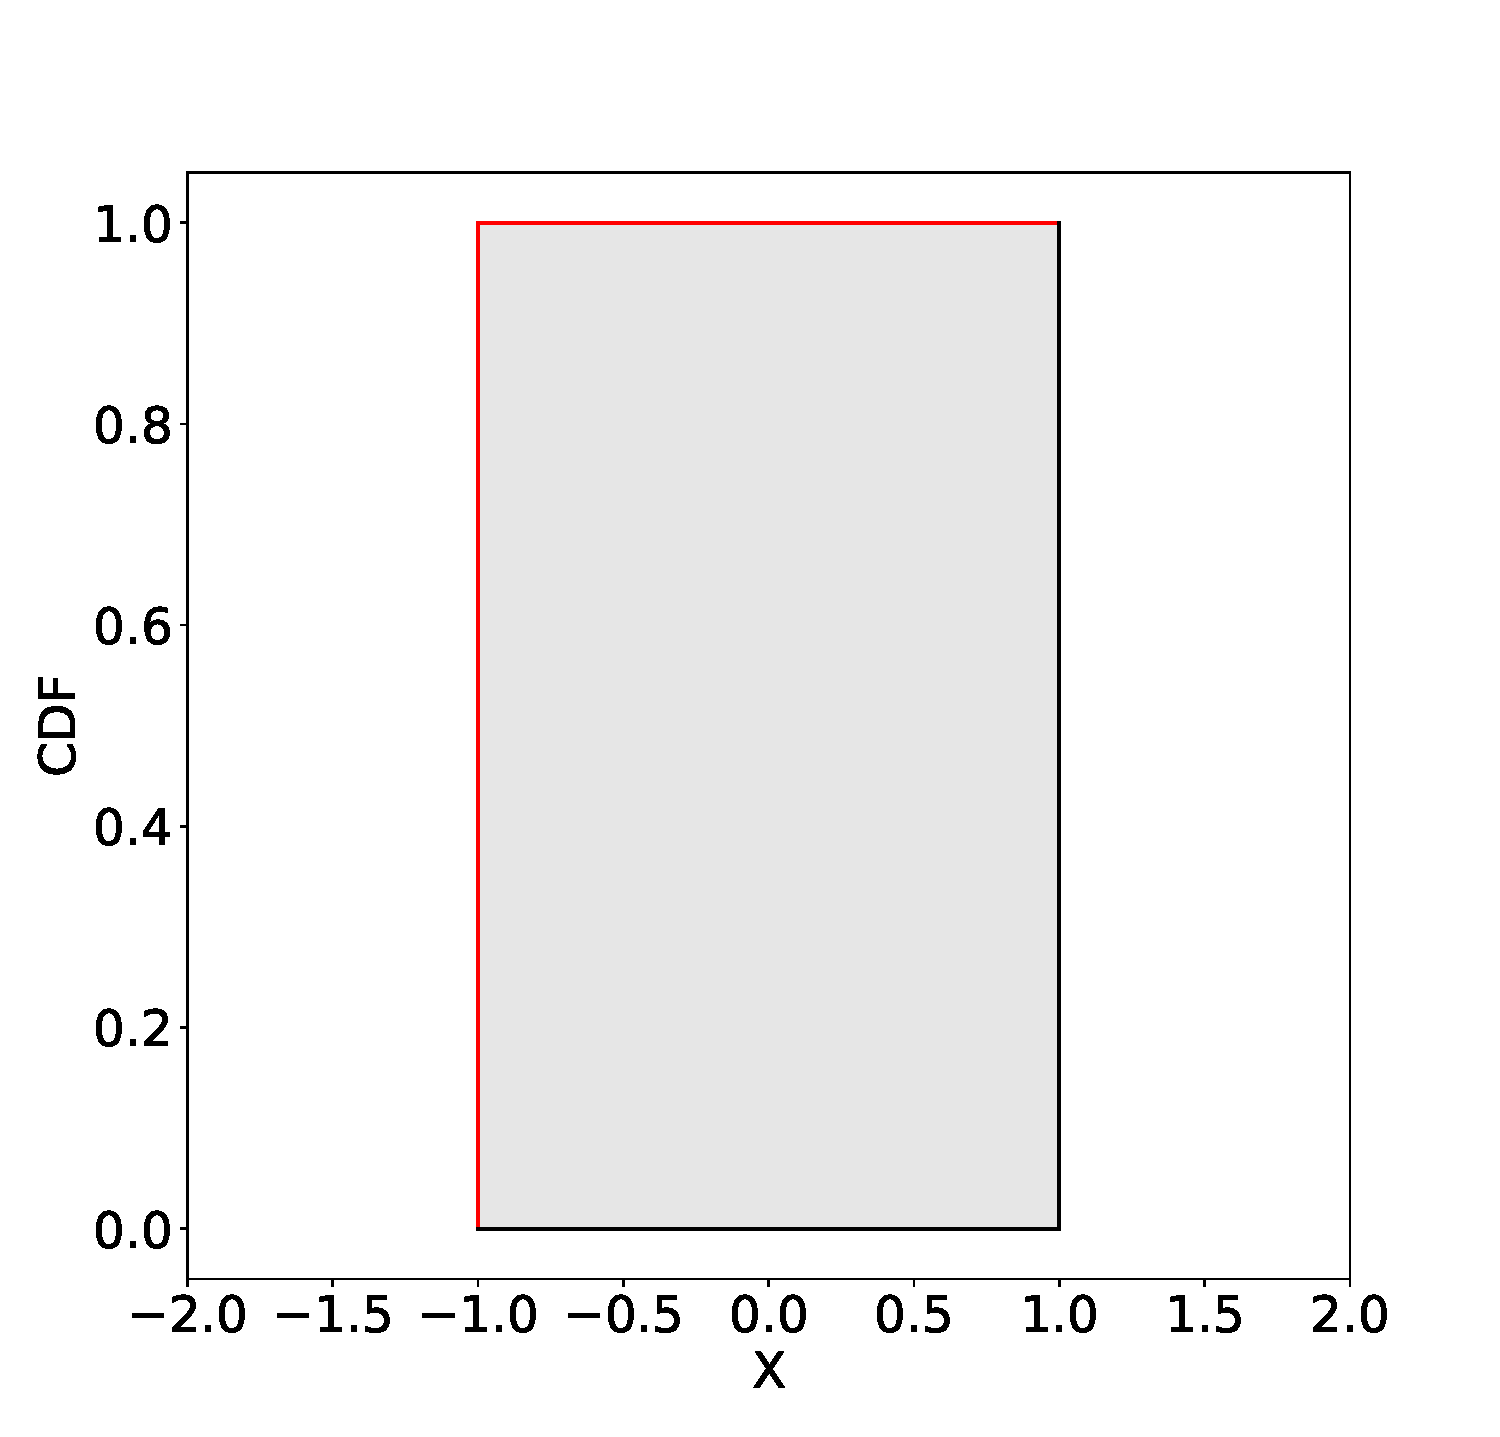
\includegraphics[width=.3\textwidth]{../examples/JuliaCon/fig1/fig1_interval.pdf}\hfill
  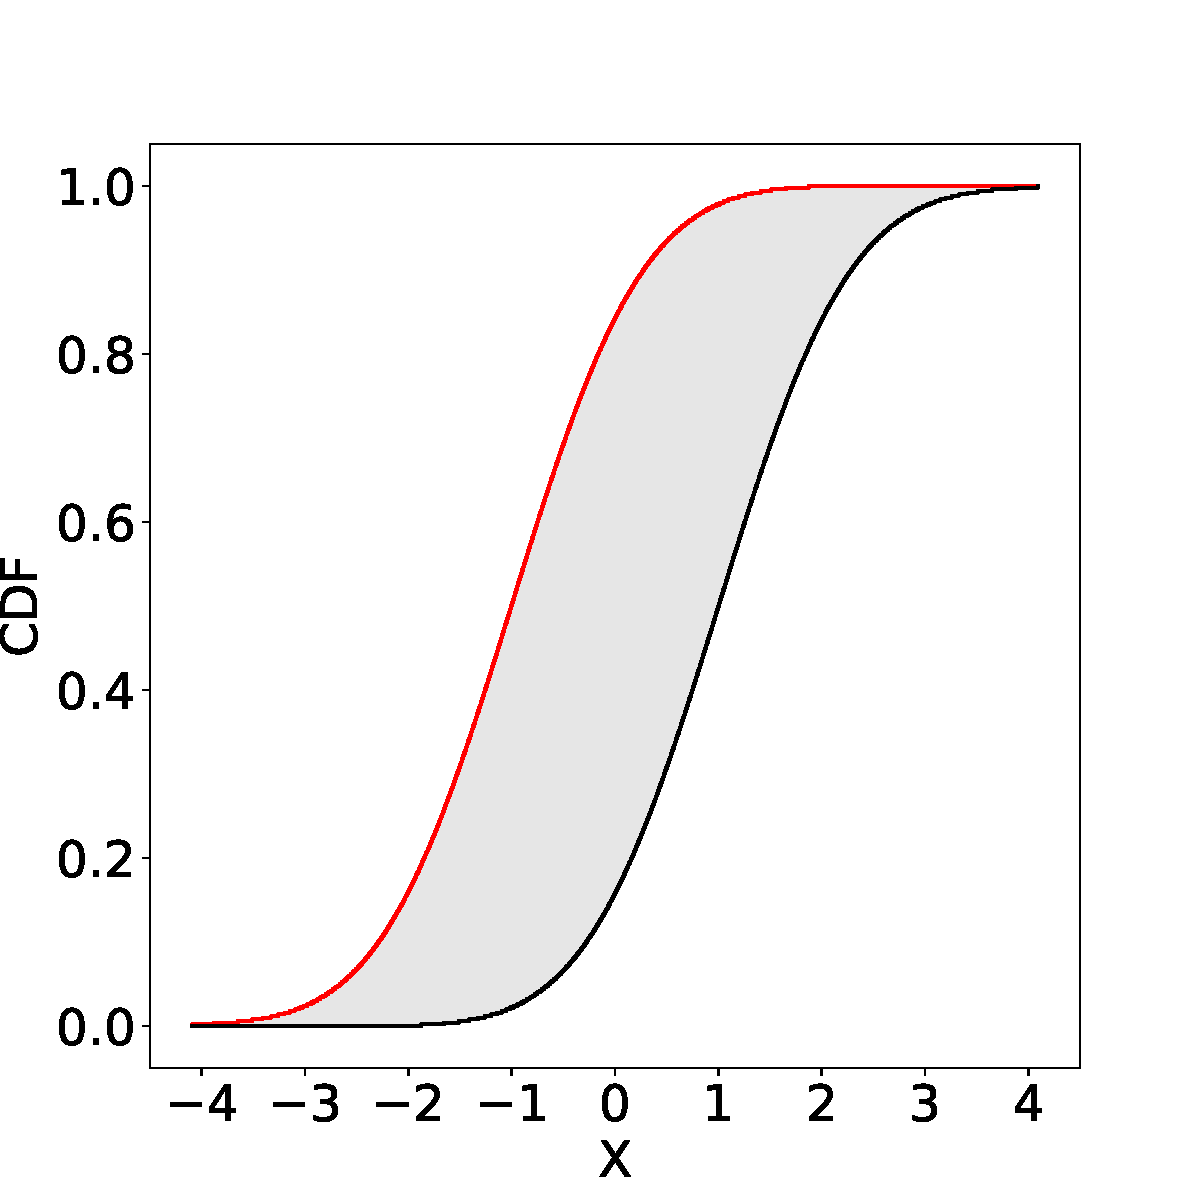
\includegraphics[width=.3\textwidth]{../examples/JuliaCon/fig1/fig1_pbox.pdf}
  
  \caption{A precise distribution, an interval and a probability box}
  \label{fig:figure1}
  
\end{figure*}

P-boxes generalise precise distributions and intervals in the following way. A distribution is a p-box with a precise cdf and moments, i.e. when: 

\begin{align*}
  \underline{F}(x) &= \overline{F}(x), \\ 
  \underline{\mu}  &= \overline{\mu}, \\ 
  \underline{\sigma}^2 &= \overline{\sigma}^2
\end{align*}

\noindent and an interval $[a,b]$ is a p-box whose bounds are step functions: 

\begin{align*}
    \underline{F}(x) &= \epsilon_{b}(x)\\
    \overline{F}(x) &= \epsilon_{a}(x) ,
\end{align*}

\noindent where $\epsilon_k$ is: 

\begin{equation*}
   \epsilon_k(x) = \begin{cases} 0 &\text{when } x < k \\ 1 &\text{when } x \geq k \end{cases}
\end{equation*}

Moreover, theoretical bounds on the mean and variance of an interval can be found [CITE SCOTT]:

\begin{align*}
  \mu &\in [a, b] \\
  \sigma^2 &\in [0, (b - a)^{2/4}]
\end{align*}

That is, it is not possible to find a distribution whose range is in $[a, b]$ and whose variance is greater than $(b-a)^{2/4}$. The lower bound on the variance is zero, since scalars are also included in the interval. Under this definition of an interval, a random sample will always be the interval $[a, b]$, the cdf returns 0 when $x < a$, the interval $[0,1]$ when $a <= x < b$, and $1$ when $b <= x$. Further, the probability measure of the interval $X = [a, b]$ will be: 

\begin{equation*}
  \mathbb{P}_{X}(U) = \begin{cases}
    0 & \text{when } U \cap [a,b] = \emptyset \\
    1 & \text{when } [a,b] \subseteq U  \\
    [0, 1] & \text{otherwise }\\
  \end{cases}
\end{equation*}

\noindent That is, if the set $U$ does not intersect the interval $X$, $\mathbb{P}_{X}=0$, i.e. $U$ certainly does not contain any of the random variables. If $X$ is fully contained in $U$, $\mathbb{P}_{X}=1$, i.e. $U$ certainly contains all of the random variables. And finally if $U$ intersects (but does not contain) $X$, the probability measure is the vacuous probability interval $\mathbb{P}_{X} = [0, 1]$, i.e. we are completely uncertain about the containment. Note that the $P_{X} = \{0, 1, [0,1]\}$ is due to the interval bounds being step functions. Generally p-boxes may yield any probability interval.

\subsection{Outer representations of p-boxes}

An important feature of probability bounds analysis is how distribution functions and p-boxes are represented. Generally, analytical solutions for cdfs are not readily available, for example the normal distribution's cdf can only be found by integrating the density, usually done with Gaussian quadrature. However, even if the functions were available analytically, when the variables are used in an arithmetic operation the output distribution will not necessarily belong to the same family. Therefore we require a representation of these continuous functions which is not dependent on the distribution family (for example Polynomial chaos expansion), and ideally is robust.

We follow the representation first introduced by Williamson and Downs \cite{williamson1990probabilistic}, where a discrete upper and lower approximations of distribution functions are constructed using the inverse cdfs. A minimal p-box structure is as follows:

\begin{lstlisting}[language = Julia]
  using IntervalArithmetic

  struct pbox{T<: Real}
    u :: Vector{T}    # right descrete inverse
    d :: Vector{T}    # left descrete inverse
    m :: Interval{T}  # interval mean
    v :: Interval{T}  # interval variance
    shape :: String   # shape
  end
\end{lstlisting}

\noindent where the vectors $u$ and $d$ are the "up" and "down", or the "left" and "right", edges of the p-box. The intervals $m$ and $v$ are the interval moments, and the $shape$ is a string containing any distribution family information.




\begin{figure*}[htp]

  \centering
  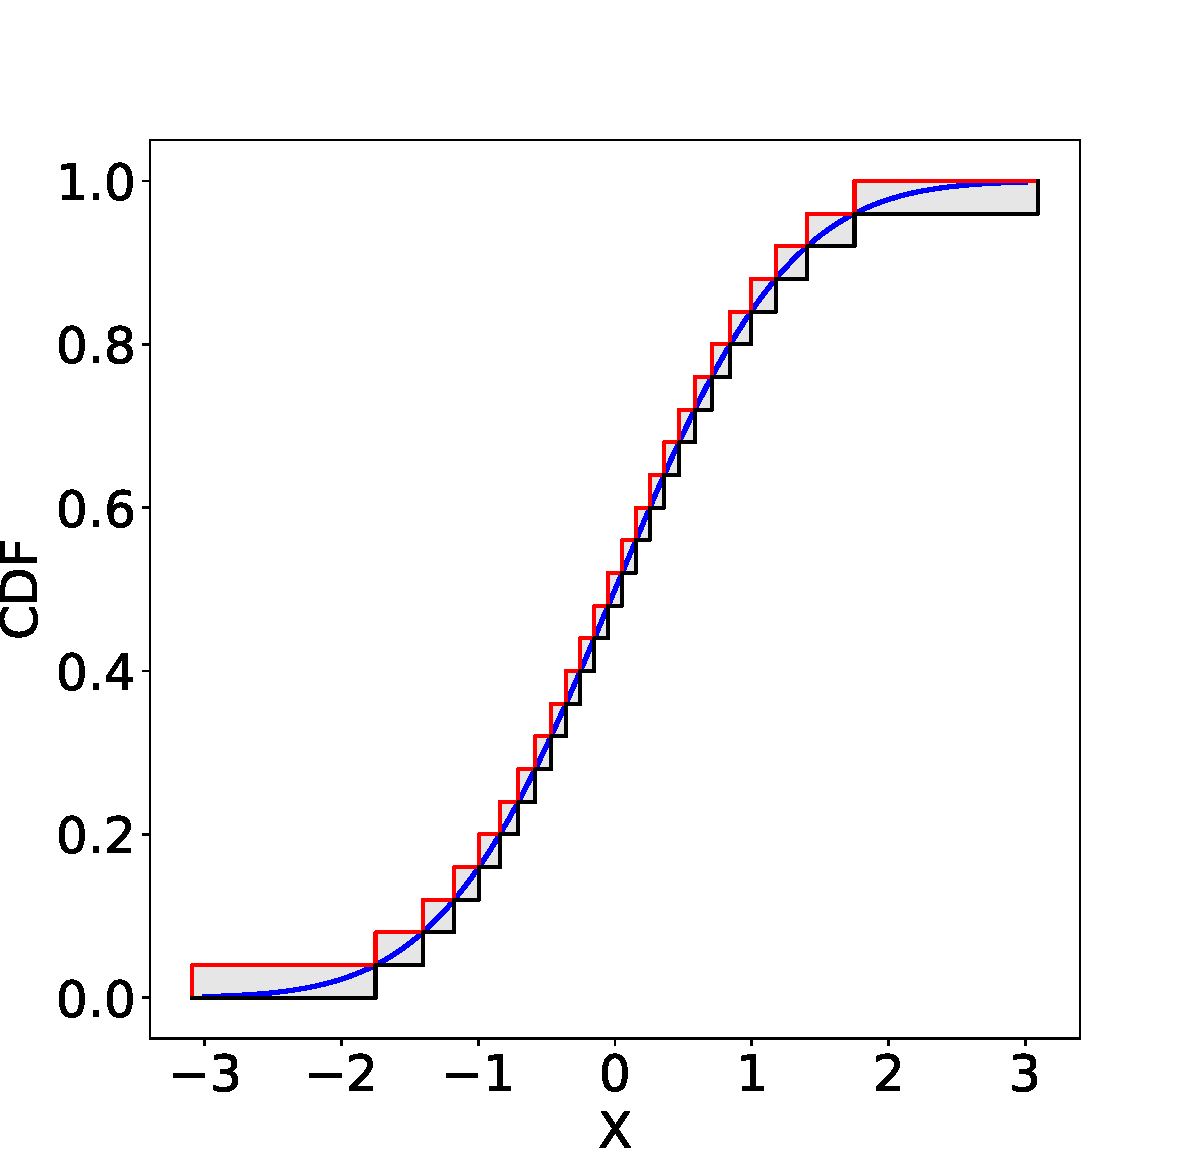
\includegraphics[width=.3\textwidth]{../examples/JuliaCon/fig2/fig2_pbox1.pdf}\hfill
  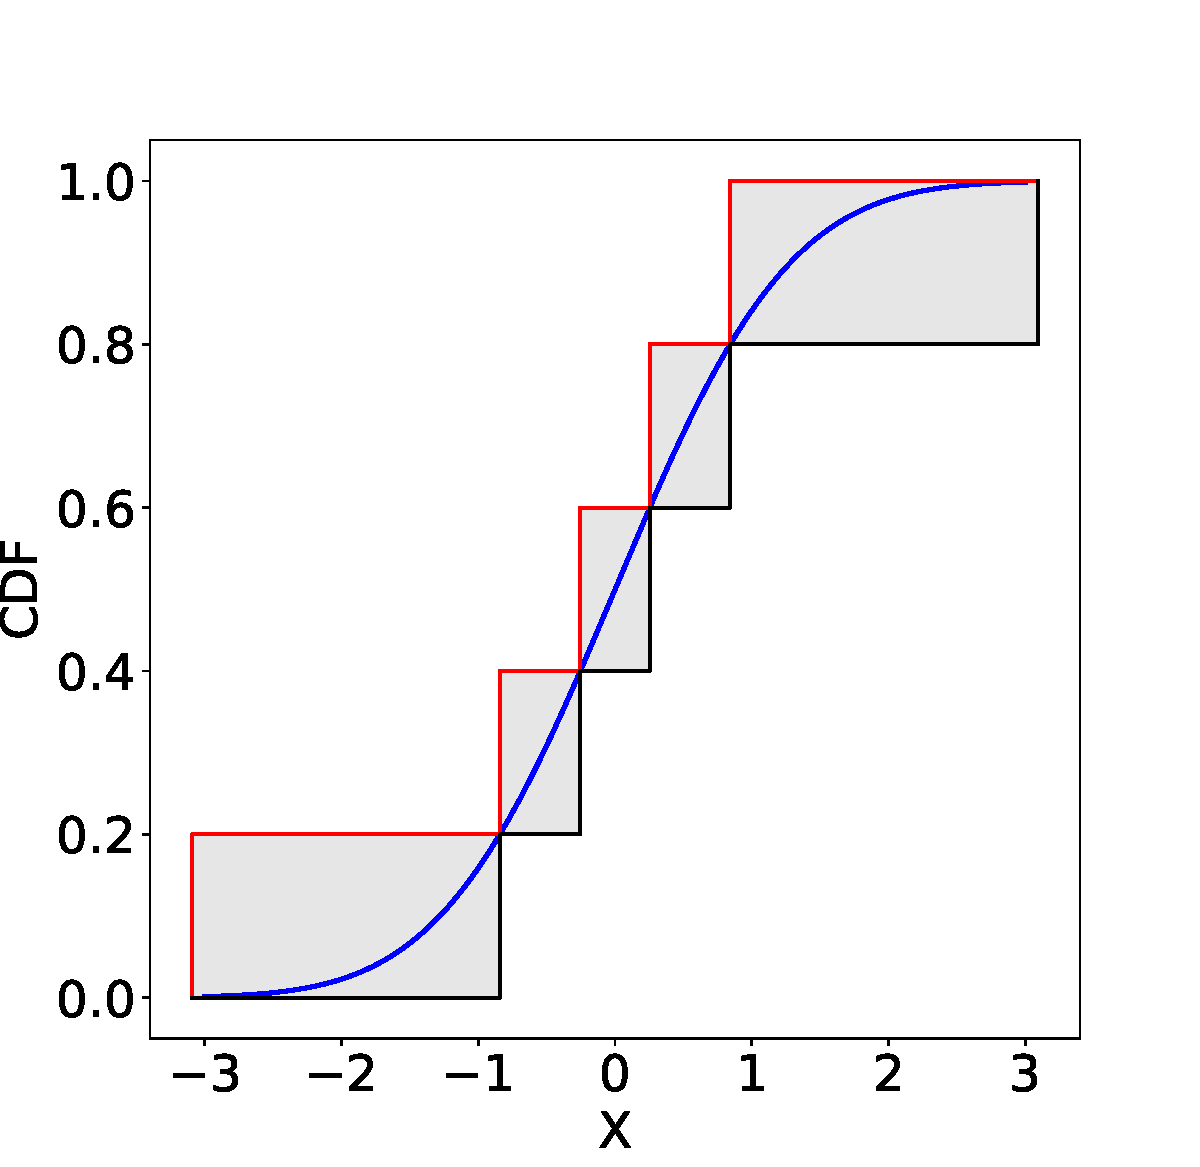
\includegraphics[width=.3\textwidth]{../examples/JuliaCon/fig2/fig2_pbox2.pdf}\hfill
  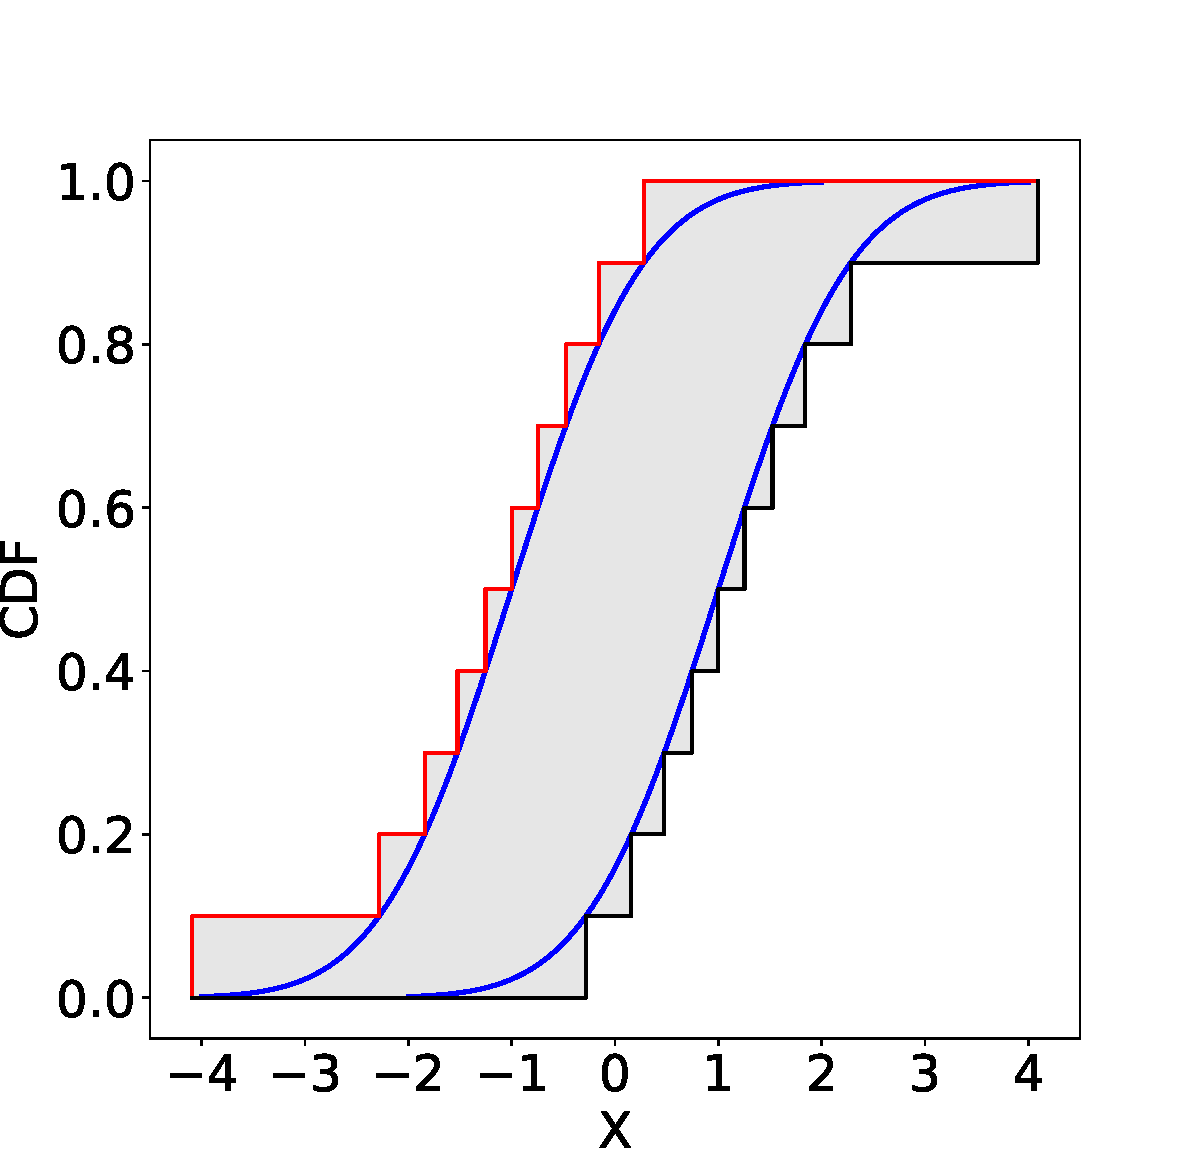
\includegraphics[width=.3\textwidth]{../examples/JuliaCon/fig2/fig2_pbox3.pdf}
  
  \caption{A precise distribution, an interval and a probability box}
  \label{fig:figure2}
  
\end{figure*}


\subsection{Where do p-boxes come from?}

In this section we discuss some situations where p-boxes arise naturally.


\subsubsection{Partial distributional information} %\hfill \break



\subsubsection{Partial moment information} %\hfill \break
\label{section:Moments}
%It is well known that a random variables distribution function cannot be 


\subsubsection{Operations involving intervals and distributions} %\hfill \break

\subsubsection{When dependencies between distributions are uknown} %\hfill \break

\subsubsection{Outer approximations of precise distributions} %\hfill \break
%P-boxes generalise intervals and distribution functions. 

\subsubsection{Inferential methods where data is limited or bad} %\hfill \break

%Probabilities are 

\subsection{Relationship to other ideas}

\subsubsection{Random set theory}

\subsubsection{Possibility theory}


%\section{Operations on p-boxes}

%\section{P boxes}

\subsection{Bivariate p-boxes}


\section{P-box arithmetic}

\subsection{Uniary operations}



\section{An uncertain programming language}
\label{sec:additional_faci}

The long term goal of such a framework is to create a fully uncertain programming language, where any computer variable may be represented as an interval, distribution, p-box or other uncertain quantity. Such a framework would allow for uncertain extensions of deterministic functions to be computed in an automatic, rigorous and tight fashion. In this section we argue why Julia is an ideal target language for such a framework, and discuss some of the remaining theoretical tasks required to make such a goal a reality. 

\section*{Acknowledgements}

The authors would like to thank the support of this work from the Engineering Physical Sciences Research Council (EPSRC) iCase studentship award. This research is funded by the EPSRC with grant number EP/R006768/1, which is acknowledged for its funding and support. This work has been carried out within the frame- work of the EUROfusion Consortium and has received funding from the Euratom research and training programme 2014–2018 and 2019–2020 under grant agreement number 633053. The views and opinions expressed herein do not necessarily reflect those of the European Commission

% **************GENERATED FILE, DO NOT EDIT**************

\bibliographystyle{juliacon}
\bibliography{ref.bib}


\end{document}

% Inspired by the International Journal of Computer Applications template
